\chapter{General discussion}
\label{ch:generaldiscussion}

\section{Contributions of this thesis}

This thesis aimed to investigate the microbial ecology and biogeography of the \ac{SO}.
To achieve this, two factors that structure the biogeographic distribution of microorganisms in the \ac{SO} were selected for study: the \ac{PF}, a major biogeographic barrier, and advection, a potentially major biogeographic force.

\subsection{The Polar Front}

This project found good evidence that the \ac{PF} is a major biogeographic barrier in the \ac{SO}, by demonstrating that the bacterial and archaeal communities in the waters to the south (the \ac{AZ}) are significantly different from the waters to the north (the \ac{SAZ} and subtropical waters north of the \ac{STF}, primarily representing \ac{SAMW}) (\secreft{ch:polarfront}).

This is not the first study on the effect of the \ac{PF} on the distribution of \ac{SO} microbiota.
Variation in the position of the \ac{ACC}, which determines the location of the \ac{PF}, has been shown to influence zooplankton composition \citep[e.g.][]{Chiba:2001un,Hunt:2001vp}, including dinoflagellates \cite{Esper:2002ui}\footnote{Interestingly, one study described the biogeographic effect of \ac{ACC}-associated fronts on zooplankton as being only weakly related to environmental parameters \cite{Ward:2003db}, suggesting the effect of advection (\secreft{ch:advection}) on zooplankton as a potential avenue for future research}.
The \ac{ACC} and/or \ac{PF} have similarly been shown to influence the distribution of Roseobacter phylotypes \cite{Selje:2004ka,Giebel:2009hr}, Flavobacteria \cite{Abell:2005ji}, and SAR11 phylotypes \cite{Giebel:2009hr}.
However, this thesis provides a significant contribution, presenting the first community-level (metagenomic) survey of \ac{SO} bacterial and archaeal plankton performed over a latitudinal transect occupying all major \ac{SO} surface water masses to give an integrated snapshot of the microbial ecology and biogeography of the \ac{SO}.

As well as the confirming previous findings on the level of individual taxonomic groups, this study found that the effect of the \ac{PF} extends to the whole community, and even to the distribution of genomically encoded functional potential.
The higher abundance south of the \ac{PF} of Bacteroidetes and Rhodobacterales, associated with the degradation of phytoplanktonic byproducts \citep[e.g.][]{Buchan:2005hd,Williams:2012gsa}, reflect the higher concentrations of (primarily eukaryotic) phytoplankton in this region. 
This was also reflected in the functional analysis, with an overrepresentation of high-specificity transporters, suggestive of copiotrophic taxa in a ``feast'' phase \cite{Lauro:2009gx}.
In general, waters south of the \ac{PF} reflected the upwelling of nutrient-rich \ac{NADW} and higher supply of light during the austral summer, which make the region significantly more active and productive than \ac{SAZ} and even subtropical waters to the north.

These northern waters were characterised by a higher relative abundance of slow-growing, nutrient-scavenging oligotrophs such as SAR11 and SAR116.
Functionally, this was reflected in the higher abundance of genes encoding branched-chain amino acid transporters, which both SAR11 and SAR116 possess.
The other significant feature of region north of the \ac{PF} was the higher abundance of the cyanobacterial genera \genus{Prochlorococcus} and \genus{Synechococcus}, and concurrently the photosynthesis functions they encode.
This was most likely due to the sensitivity of these genera to temperature.

\subsubsection{Biogeographic role of the Polar Front}

Having shown that the \ac{PF} is a major biogeographic barrier, and in light of the advection study also presented in this thesis (\secreft{ch:advection}), it is worth considering the mechanism(s) by which the \ac{PF} shapes microbial biogeography.
It is likely that three main forces are at work.

The first is the role of the \ac{PF} as a ``biogeographic barrier'' in the classical sense in which the term is applied to macroorganisms.
In other words, it physically prevents or slows the migration of cells between the regions it divides, leading if not to allopatric speciation, at least to some degree of genomic divergence, which is amplified by the differences in environmental properties.
\citet{Selje:2004ka}, who first reported that \ac{RCA} phylotypes differed across the \ac{PF}, offered this mechanism as a likely explanation, and they have been echoed by further reports on RCA \cite{Giebel:2009hr} and Flavobacteria \cite{Abell:2005ji}.
The advection effect (\secreft{ch:advection}) supports such a mechanism, by showing that oceanic regions poorly connected by advection (i.e.\ poorly mixed) have less similar microbial communities.

The second mechanism, complementary to the first, is the difference in physicochemical properties resulting from the same oceanographic forces that create the \ac{PF}: in particular, the advective distribution of nutrients.
The ratio of biological N/P export in \ac{SO} surface waters increases northwards from the region of upwelling \ac{CDW} in the \ac{AZ} (N/P\textsubscript{exp} \textless{} 16) to the \ac{SAZ} (N/P\textsubscript{exp} \textgreater{} 16) \cite{Weber:2010fi}.
This directly contradicts the standard assumption that \ce{PO4^3-} is exported to the deep ocean in a fixed proportion of \textapprox{}16:1 available \ce{NO3^-} to \ce{PO4^3-} (the Redfield ratio).
\citet{Weber:2010fi} convincingly showed that this is largely a result of the biogeographic distribution of low cellular N/P diatoms relative to other high cellular N/P plankton.
The distribution of diatoms in the \ac{SO} is in turn controlled by the concentration of silicic acid \cite{MFranck:2000kt}, which supplied in abundance south of the \ac{PF} by upwelling \ac{CDW} but is limiting further north \citep[widely held, but well summarised by][]{Coale:2004to}, explaining the observed difference in N/P\textsubscript{exp}.
Further, \citet{Weber:2010fi} showed that advective mixing of organic N and P exported to the deep ocean by sinking organic matter and remineralised in the aphotic zone was sufficient to counterbalance the differential export of N and P by diatoms and other plankton, leading to an equilibrium approximately equivalent to the Redfield ratio of 16:1 N:P.
Advective transport of nutrients and the distribution of plankton are thus intimately connected in the \ac{SO}, with the \ac{PF} acting as a key barrier between the nutrient-rich \ac{AZ} upwelling and the comparatively oligotrophic \ac{SAZ}.
As well as the distribution of major nutrients (N, P and Si), the waters to the north and south of the \ac{PF} differ in temperature and salinity due to their different circulatory origins \cite{Foldvik:1988gp}.

The third mechanism by which the \ac{PF} may act as a biogeographic boundary is more mundane.
Being a polar ocean, the \ac{SO} is subject to strong latitudinal gradients in air temperature and sunlight unrelated to its oceanographic structure.
The Antarctic Circle, the latitude at which continuous 24-hour periods of sunlight (and of darkness) become possible, is considerably south of the \ac{PF} (\textapprox{}66.5\textdegree{} S, although this varies due to slow changes in the Earth's axial tilt).
However, the existence of large environmental gradients means that longitudinal features (fronts, currents, divergences and convergences in both the ocean and atmosphere) are almost certain to be associated with biological discontinuities simply by virtue of lying on a particular latitude, without necessarily having any causal relationship.
In the case of the \ac{PF} and its role in the distribution of marine bacteria and archaea, the possibility that this was the only significance of the \ac{PF} was explicitly tested for and discounted in this study: other arbitrary latitudinal lines do not structure the biological observations as well as the \ac{PF} (see \secreft{ch:polarfront}).
Nevertheless, it is likely that latitudinal gradients not directly related to the \ac{PF} (particularly sunlight) do make some contribution to the biogeographic pattern.

\subsection{The advection effect}

The second major focus of this thesis was the role of advection in shaping the biogeography of microorganisms in the \ac{SO}, and by extension the ocean in general.
This question is highly topical, given the recent discovery that geographic distance often controls microbial biogeography in contradiction with the Baas Becking hypothesis (key studies: \citet{Cho:2000tn,Whitaker:2003dz}; reviews: \citet{Martiny:2006jy,Hanson:2012cb}), and the frequent invocation of circulation to explain observed distributions of marine microbes \citep[e.g.][]{Lauro:2007bf,Giebel:2009hr,Ghiglione:2012ei,Sul:2013in}.

Previous work addressing this question has focused on water mass endemicity and qualitative descriptions of circulation.
\citet{Galand:2009hy} and \citet{Agogue:2011fm} presented evidence of the specificity of microbial communities to water masses in the Arctic and North Atlantic oceans, even across small geographic distances, suggesting boundaries between water masses act as biogeographic barriers, although these observations do not exclude simple environmental selection.
\citet{Hamilton:2008tp}, also describing the Arctic and North Atlantic oceans, found picoeukaryotic communities clustered by circulatory origin as determined by qualitative analysis of hydrographic properties.
The authors noted that quantitative modelling of circulation would be necessary to directly test the role of circulation.
Recently, \citet{Hamdan:2013ko} demonstrated a similar clustering of prokaryotes Arctic marine sediments with their circulatory origins.
Both studies controlled for environmental factors to various degrees.

This thesis (and the associated publication) present the first quantitative test of the effect of advection on microbial biogeography.
By employing a high-resolution computational model of \ac{SO} circulation to determine advective distances between samples, the standard ecological tools of distance matrices and partitioning of variance with the partial Mantel test could be used to isolate the effect of advection from environmental selection and spatial separation.
This thesis thus also contributes a replicable method for future studies to evaluate the advection effect in other marine environments and compare it against other biogeographic forces.

Together, contemporary environmental selection and geographic distance explain \textapprox{} 50\% of variation in microbial community composition \cite{Hanson:2012cb}.
In this study, advection was estimated to explain 7\% of variation \figref{fig:biogeographybarchart}.
This is a conservative estimate, as higher value were found when alternative distance metrics were considered and problematic samples excluded, and samples which shared a common advective origin but had a large mutual advective distance were not considered.
Future work on the advection effect will be valuable not only in confirming its role but in obtaining an accurate measure of its magnitude.

\begin{figure}
  \centering
  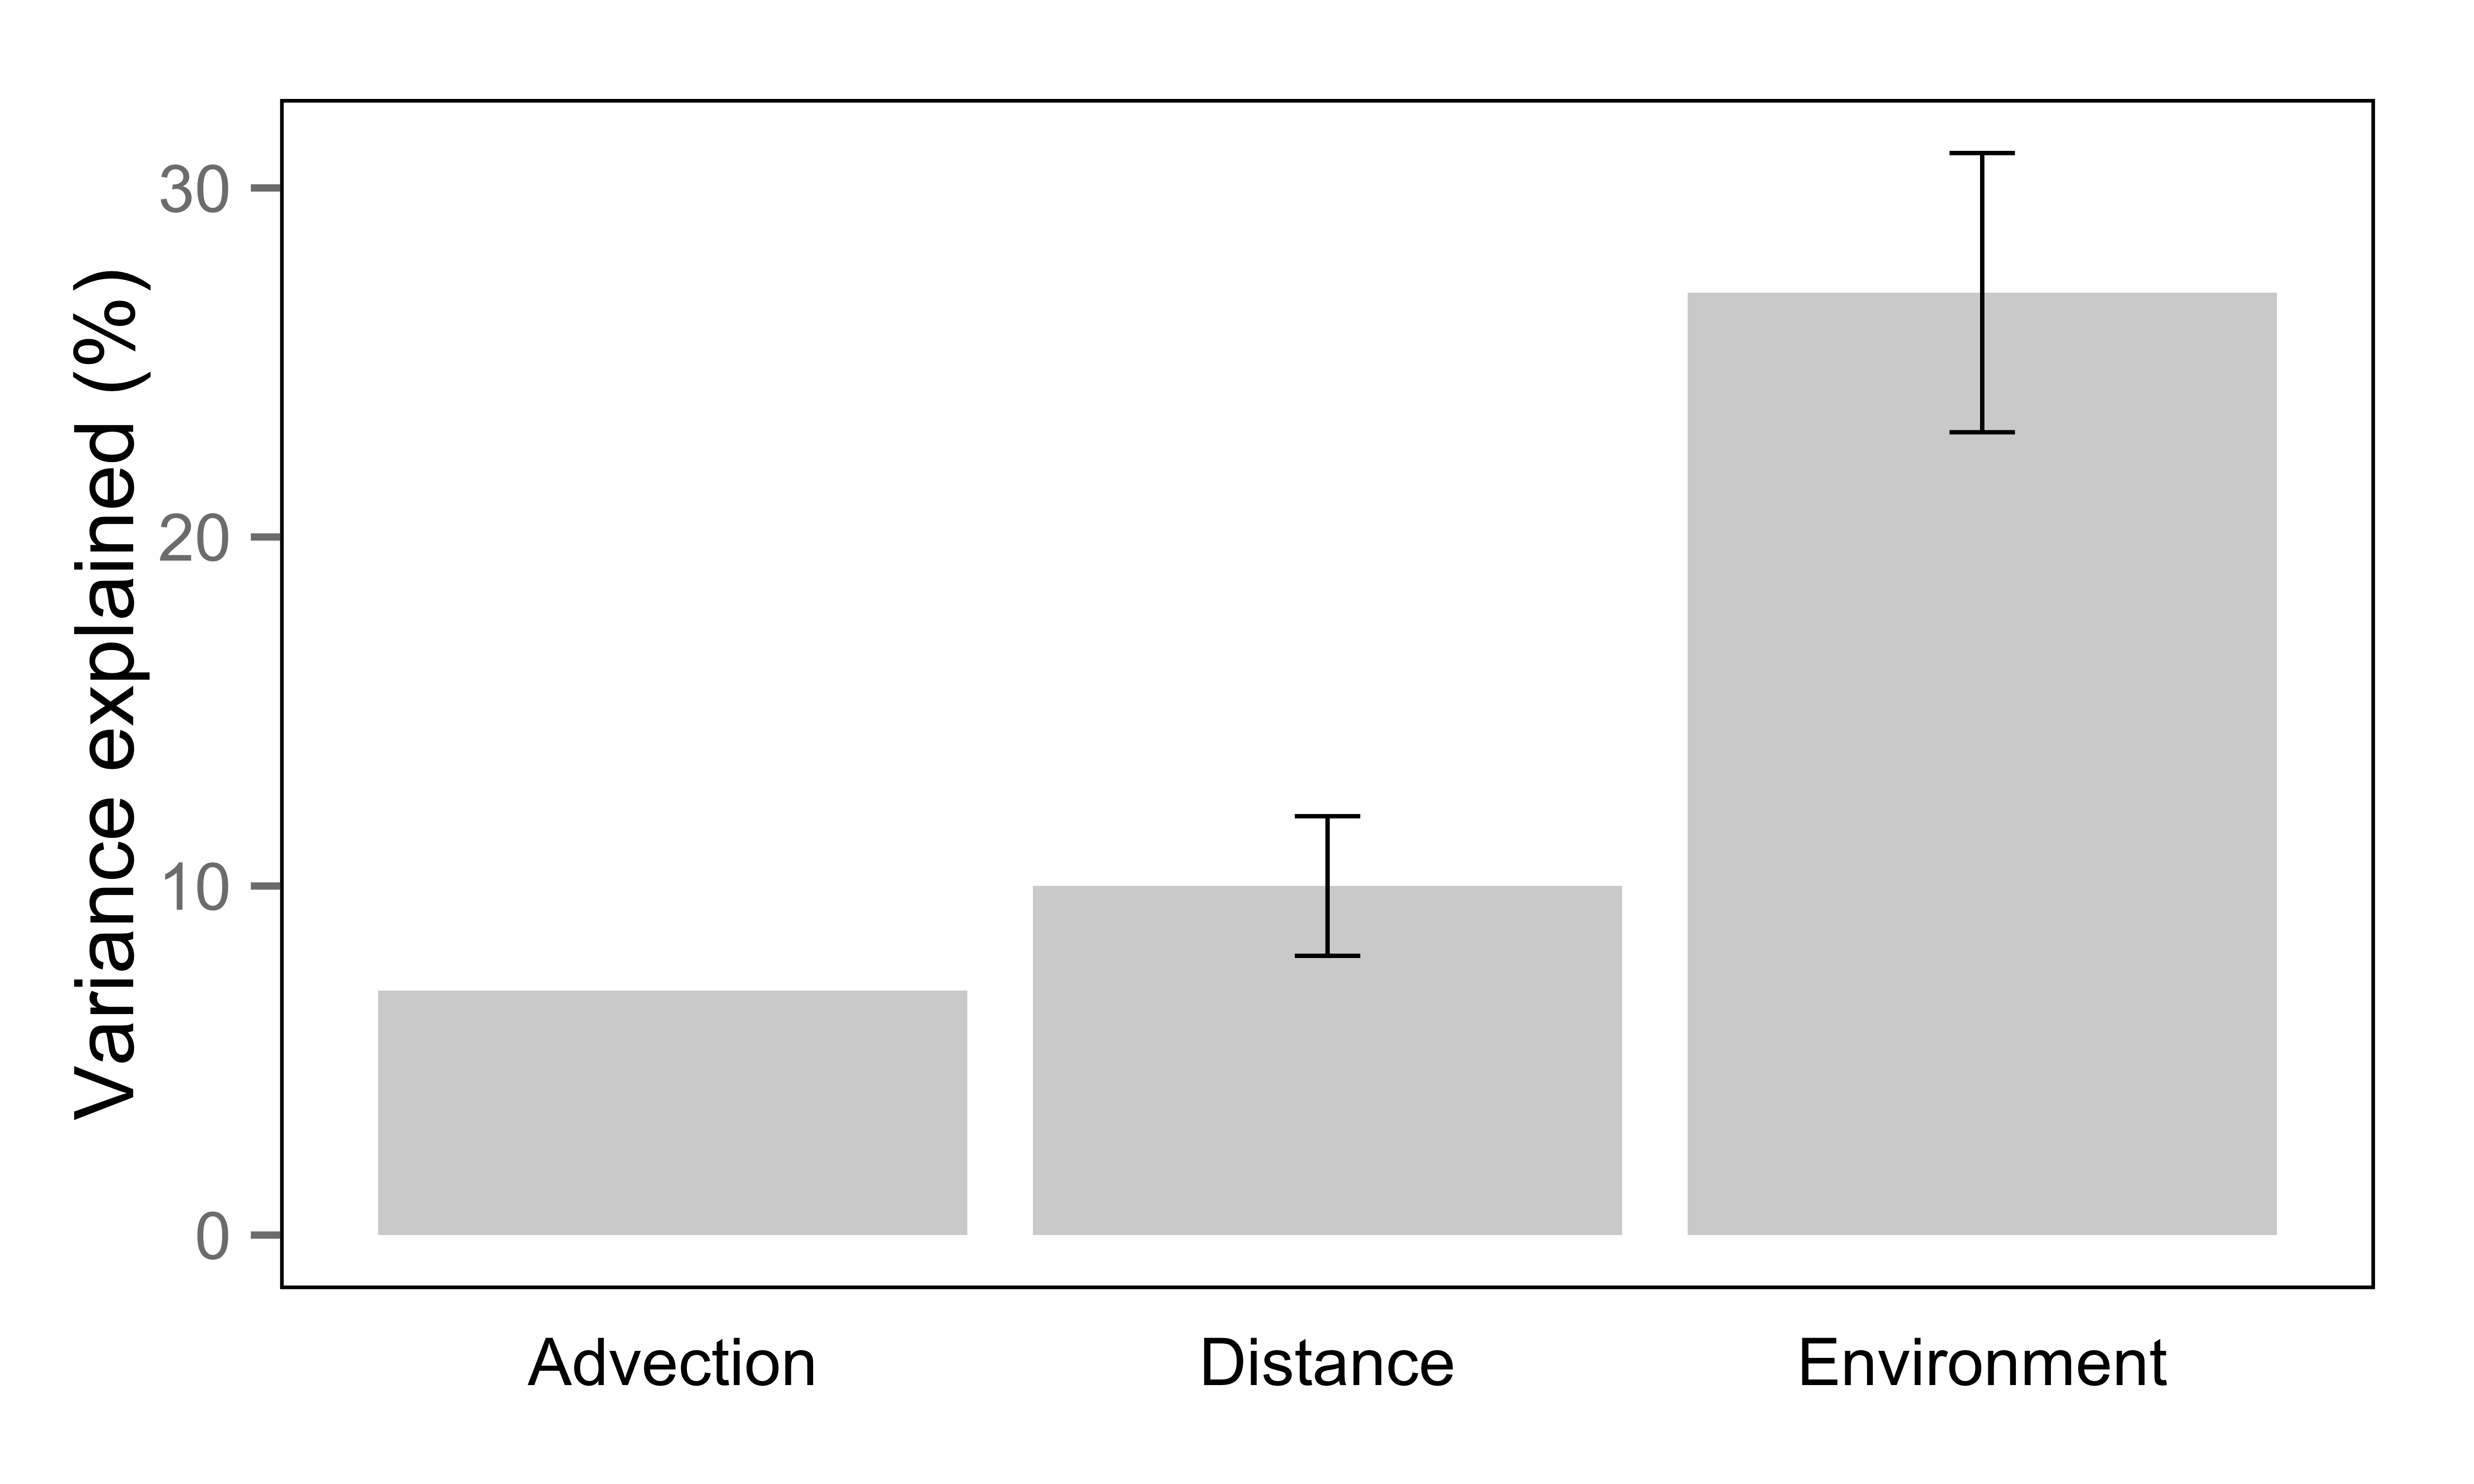
\includegraphics[width=\textwidth]{../generaldiscussion/biogeographybarchart.png}
  \caption[Biogeographic effect sizes]{Variation in microbial community composition explained by environment and distance effects (data from review of 19 studies by \citet{Hanson:2012cb}; error bars represent standard error) and by the advection effect (this study).}
  \label{fig:biogeographybarchart}
\end{figure}


\subsection{\softwarename{minspec}}

This thesis also presents a novel software tool, \softwarename{minspec}, which contributes to improving the accuracy of \ac{OTU} assignment and calculation of relative abundances in metagenomic studies.

The number of publicly available full genome sequences for microbial species is growing exponentially: over the course of this project, the number of microbial genomes in the RefSeq database increased from 5,500 (May 2010) to 15,000 (March 2013) (\url{http://www.ncbi.nlm.nih.gov/refseq/statistics/}, accessed 12 April 2013).
As more genomes become available, the number of potential high-quality matches to a given metagenomic read will increase as a natural result of genomic identity between related organisms.
\softwarename{minspec} reduces the need to rely on nucleotide identity as the sole objective standard for assigning metagenomic reads to \acp{OTU}, making use of the contextual information provided by the full set of reads to inform the assignment of each individual read.
While assembly of metagenomic reads can to some extent perform the same function \cite{Temperton:2012fj}, \softwarename{minspec} does not require long or overlapping reads, making it well-suited to the short read lengths of current next-generation sequencing methods and to environments such as the open ocean that have a long tail of low-abundance taxa.

In the long term, single-cell genomic sequencing is the most promising approach for accurate and reliable environmental genomics \cite{Blainey:2013dp}.
Until then, \softwarename{minspec} may be of use in improving the quality of metagenomic results.

\section{Levels of description in microbial ecology and biogeography}

"Top down" vs "bottom up": medicine started "top down"; economics started "bottom up"; microbial ecology would like to have started "top down", but methodologically was forced to proceed "bottom up".

'omics finally allows microbial ecology to become a "top down" discipline. But as this perspective is almost brand new, we're struggling with how to meaningfully carve up and interpret what we see. The species concepts seems natural and easily measured on the cells-and-petri-dishes level, but seems to become almost meaningless when examining a whole community. Moreover, the tiny size, incredible diversity and adaptiveness of microbes means enormous amounts of data must be collected and carefully processed to identify even the simplest of biogeographic patterns (e.g. distance effect).

climate change needs a mention here somewhere

Nevertheless, progress is being made: environment effect, distance effect, and now advection effect. The challenge is linking the top to the bottom. It's very hard to disentangle the effects of individual OTUs — give as examples surface vs. DCM; BVSTEP of advection results. Just as it might be misguided for a physician to try to conceptualise a disease in terms of the elemental ratios of diseased vs healthy tissue, it may not even be a fruitful approach to try and think of ecological patterns in terms of their constituent species.

Future work

SO microbial ecology
Current metagenomic methods require only looking at a small part of the community at a time (constrained by primer selection, size fractionation) - would be great to see the whole thing - single cell?

Future studies should seek to confirm the advection results, particularly the advection effect, in other regions.
